\documentclass[tikz, preview]{standalone}

\usepackage{amsfonts, amsthm, amssymb, amsmath, stmaryrd, etoolbox}
\usepackage{tikz}
\usetikzlibrary{matrix,arrows}

\begin{document}
\[
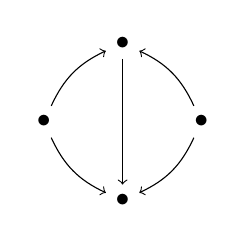
\begin{tikzpicture}
\node (a) at (0,1) {$\bullet$};
\node (b) at (1,0) {$\bullet$};
\node (c) at (0,-1) {$\bullet$};
\node (d) at (-1,0) {$\bullet$};
%
\path [<-] (a) edge[bend left=20] (b);
\path [->] (b) edge[bend left=20] (c);
\path [<-] (c) edge[bend left=20] (d);
\path [->] (d) edge[bend left=20] (a);
\path [->] (a) edge[] (c);
\end{tikzpicture}
\]

\end{document}